\noindent

\includegraphics[height=1.25cm]{images/pictograms/benchmark}

\includegraphics[height=1.25cm]{images/pictograms/under_construction}

\includegraphics[height=1.25cm]{images/pictograms/FEM}

%%%%%%%%%%%%%%%%%%%%%%%%%%%%%%%%%%%%%%%%%%%%%%%%%%%%%%%%%%%%%%%%%%%%%%%%%%%%%%%%%%%%%%%%%%%%%%%%%%%

\begin{flushright} {\tiny {\color{gray} python\_codes/fieldstone\_176/text.tex}} \end{flushright}

%\lstinputlisting[language=bash,basicstyle=\small]{python_codes/template_keywords.key}

\par\noindent\rule{\textwidth}{0.4pt}

\begin{center}
\inpython
{\small Code: \url{https://github.com/cedrict/fieldstone/tree/master/python_codes/fieldstone_176}}
\end{center}

\par\noindent\rule{\textwidth}{0.4pt}

Last revision: July. 20th, 2026.

\par\noindent\rule{\textwidth}{0.4pt}

%%%%%%%%%%%%%%%%%%%%%%%%%%%%%%%%%%%%%%%%%%%%%%%%%%%%%%%%%%%%%%%%%%%%%%%%%%%%%%%%%%%%%%%%%%%%%%%%%%%


\begin{center}
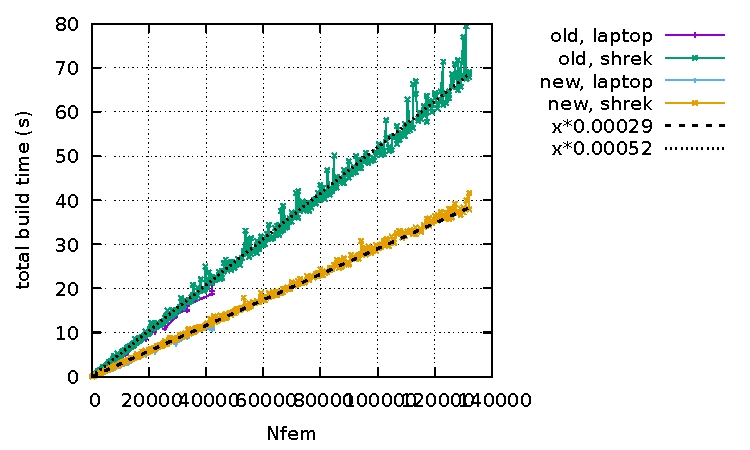
\includegraphics[width=8cm]{python_codes/fieldstone_176/results/build.pdf}
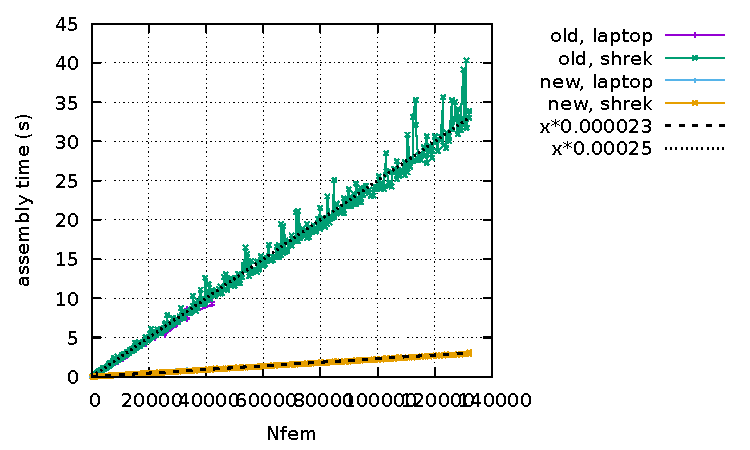
\includegraphics[width=8cm]{python_codes/fieldstone_176/results/assembly.pdf}\\
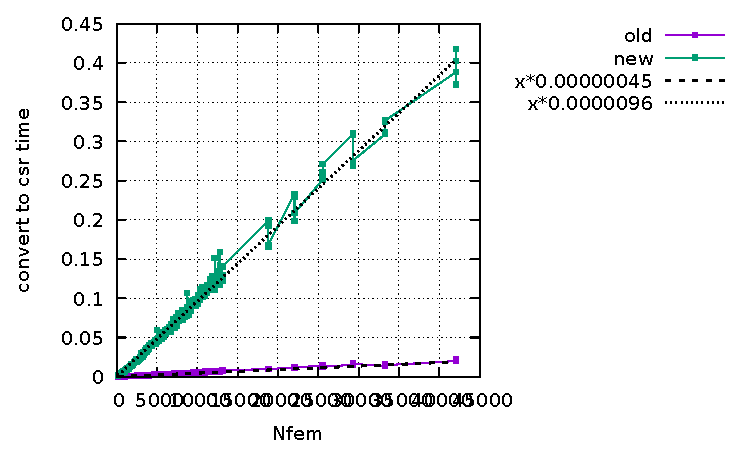
\includegraphics[width=8cm]{python_codes/fieldstone_176/results/convert2csr.pdf}
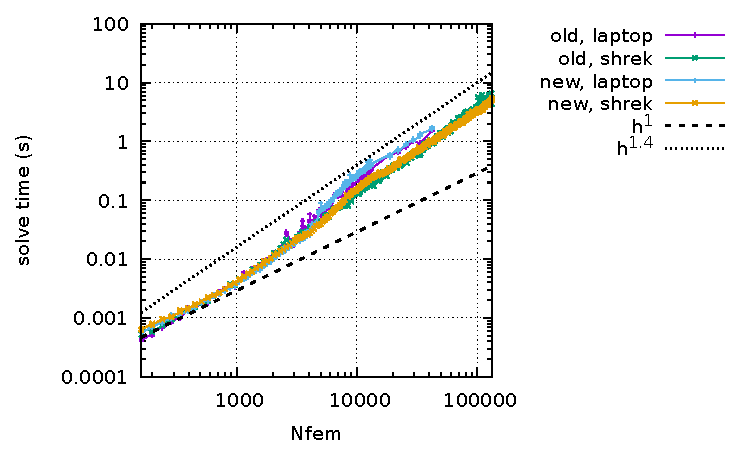
\includegraphics[width=8cm]{python_codes/fieldstone_176/results/solve.pdf}\\
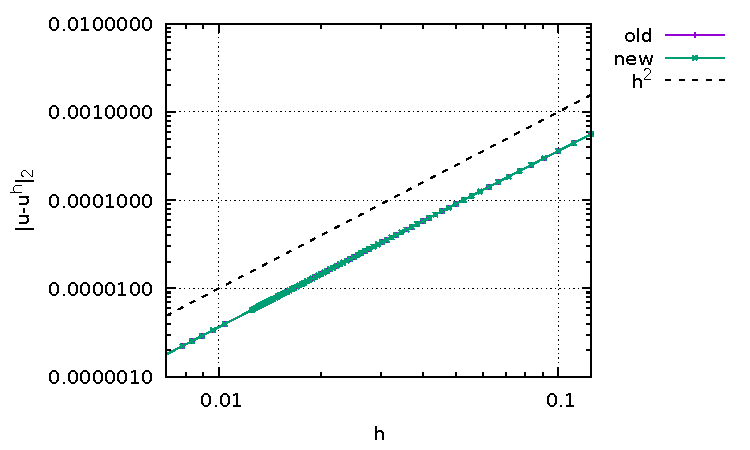
\includegraphics[width=8cm]{python_codes/fieldstone_176/results/errv.pdf}
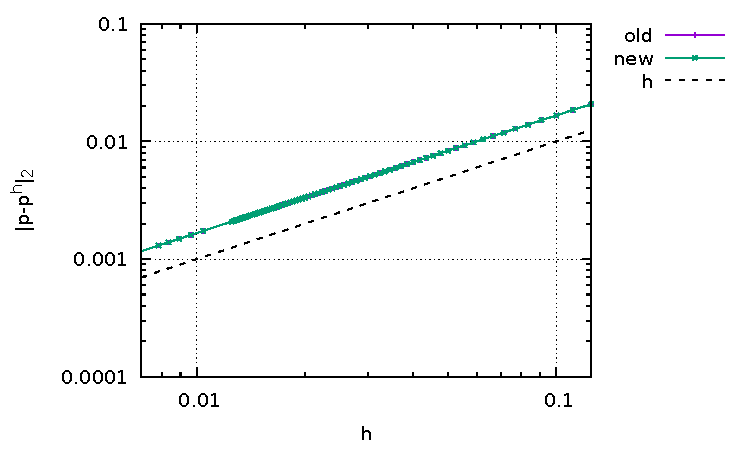
\includegraphics[width=8cm]{python_codes/fieldstone_176/results/errp.pdf}
\end{center}
